%srj
%aum gaanathipathaye namaha


\begin{figure}[t]
\begin{center}%\vspace{-1mm}
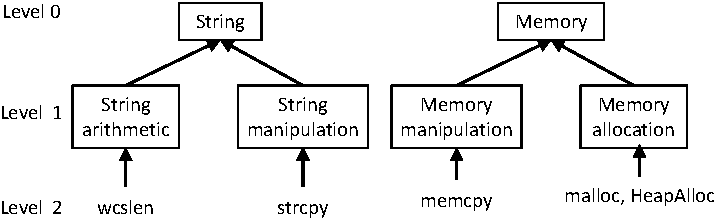
\includegraphics[width=0.4\textwidth]{srj-figures/srj-abs-1.pdf}
%\vspace{-1mm}
\caption{Library function abstraction levels}
\label{fig:abs} \vspace{-2mm}
\end{center}
\end{figure}

\section{Function Filtering}\label{sec:prefilter}

In practise, %to effectively search for a semantically similar function from a pool of several hundred thousand (or more) target functions compiled for various architectures and OS using different types of compilers with varying optimization levels,
to deal with a huge number of target functions in real-world binaries, an effective filtering process is critical such that irrelevant target functions can be removed before the expensive matching step. To this end, we leverage on three types of filters, starting from the specific one to the most general one in terms of filtering criteria, to shortlist the candidate target functions.

\textbf{Filter 1}: The first type of filters %\xyx{(\textit{aka.,} precise)}
 looks for identical library call invocations in the target functions according to the signature function. If the identical invocations are found, the corresponding targets functions are good candidates for further matching. The reason is that the library call invocations provide the semantics of the high-level function behavior.

However, this filter is OS dependent and fails to support library calls that have different names yet with similar functionality (e.g., \texttt{memcpy} and \texttt{memmove}).
%Library calls can be inlined by the compiler or programmers might implement the same functionality in user-defined functions. Thus, relying on library call names will fail. %In addition, the given function may not invoke any library call at all, in such situations, library call based filtering is not helpful.

\textbf{Filter 2}: To address the problem in library call name matching, we consider the library call operation types, which help to match the high-level functionality of the library calls. As shown in Fig.~\ref{fig:abs}, there are several ways of abstracting the functionality of a library call. Abstraction level 0 gives the base operation type (e.g., \textit{string} operation), while level 1 gives a more concrete but general abstraction supported cross all OSs.
<<<<<<< .mine
For example, \texttt{strcpy} and \texttt{strcat} can be mapped to \textit{string manipulation} operation. Therefore, we adopt abstraction level 1 to summarize the library function behavior. In addition, filter 2 is OS neutral, where functions that perform similar task but with different names across OS are mapped to the same operation type, e.g., \texttt{malloc} (Windows/Linux) and \texttt{HeapAlloc} (Windows) are mapped to \emph{memory allocation} operation type as shown in Fig.~\ref{fig:abs}.  
||||||| .r3669
For example, \texttt{strcpy} and \texttt{strcat} can be mapped to \textit{string manipulation} operation. Therefore, we adopt abstraction level 1 to summarize the library function behavior. \mahin{In addition, filter 2 is OS neutral, where functions that perform similar task but with different names across OS are mapped to the same operation type, e.g., \texttt{malloc} (Windows/Linux) and \texttt{HeapAlloc} (Windows) are mapped to \emph{memory allocation} operation type as shown in Fig.~\ref{fig:abs}}.  
=======
For example, \texttt{strcpy} and \texttt{strcat} can be mapped to \textit{string manipulation} operation. Therefore, we adopt abstraction level 1 to summarize the library function behavior. \mahin{In addition, filter 2 is OS neutral, where functions that perform similar task but with different names across OS are mapped to the same operation type, e.g., \texttt{malloc} (Windows/Linux) and \texttt{HeapAlloc} (Windows) are mapped to \emph{memory allocation} operation type as shown in Fig.~\ref{fig:abs}}.
>>>>>>> .r3679
%\ly{I want to highlight this filter 2 is OS neatural and use one example to show it in fig 4. Also we should say we maintain the mapping ourself.}
%in this study.
%\todo{Include example for op. type mapping}

However, library calls can be inlined by the compiler or programmers might implement the same functionality in user-defined functions. Thus, relying on library call names or the operation type will fail. To address this, we propose filter 3.%In addition, the given function may not invoke any library call at all, in such situations, library call based filtering is not helpful.


\textbf{Filter 3}: %To address these serious issues of the first two filters, we \xyx{propose}
The third filter is designed \xyx{to utilize} similarities in the instruction types involved in a binary function as a whole. Here, instruction type refers to a high-level operation carried out by an instruction~\cite{kruegel2005polymorphic}. In total, instructions are categorized into 14 and 8 instruction types for Intel and ARM architectures, respectively. For example, \texttt{mov} instruction is mapped to \textit{data movement} instruction type while \texttt{push} is mapped to \textit{stack operation}.
In addition, instruction types also support cross-architecture function matching, where assembly instructions from ARM and Intel architectures are mapped to the same instruction type even though they are not identical at the instruction level (e.g., \texttt{call} (Intel) and \texttt{bl} (ARM) can be mapped to \textit{invoke function} instruction type).

Nevertheless, this filter may suffer from the problem of semantics matching --- the instruction types used to implement the functions might look very similar even though they have totally different functionalities at a higher level.
Since the filtering process is to shortlist all the target functions that are similar to the signature. %, and hence similarity at the instruction level is also very relevant even though they might be different at the high-level function behaviour.
%This conservative approach is adapted not to miss any potential target functions.
For the propose of not missing any potential target functions, some semantically irrelevant functions are tolerated.

Filter 1 is specific and OS dependent. Filter 2 and 3 are general and cross-OS and cross-architecture.
Our filtering process is shown in Algorithm~\ref{algo:pre-filt}. Following the design of applying the filters one by one from the most specific one to the general one, we set the weights ($w_1 > w_2 > w_3 >0$ ) to the similarities achieved by Filter 1 to 3. At line 12, we sort the candidate functions according to the overall similarity on three filters (calculated at line 10). Finally, at line 13, we get the top $N$ of the sorting results and use them for function model matching.
%\xyx{\textbf{give concrete value in implementation, discuss about the weight set in threat to validity!}}% where filter 1 is the most precise with  $w_1=1.0$, and filter 3 is the least precise with $w_3=0.5$ while filter 2 being in the middle with $w_2=0.8$.
Note that our filtering process is performed after selective inlining step, \xyx{so} we keep a mapping from the candidate function to its invoked libraries in order to apply the filters.
%\todo{mention how NDSS 2016 gonna fail in pre-filtering}, \xyx{Mahin, maybe we can put all the comparison with NDSS paper in related work.}

%sIn addition, we use inlined target functions, which helps to

%It is important to note that, for each library call, we obtain the corresponding instruction types from the actual implementation of that library function in \texttt{libc} and \texttt{msvcrt}, for Linux and Windows binaries, respectively.


%To make \tool capable of analyzing cross-OS binaries, we use a multi-level abstraction function $\mathtt{abstractSystemAPI}$ at line \ref{algo2:abAPI} to abstract system APIs based on their type. For example, the system API (or library call) \texttt{strlen} deals with string objects, and hence  the API can be naturally abstracted to `string' type. To this end, we use two levels of granularity (i.e., level 0 and 1) to abstract the system APIs, where each abstraction level play a different role in \tool~ --- abstraction level 0 abstracts the system API to their basic type, whereas level 1 provides more meaningful information about the API. For example, using our abstraction function, the system APIs \texttt{strlen}, \texttt{strcpy} and \texttt{strncpy} can be abstracted into two levels shown in Fig.~\ref{fig:abs}.


%Based on the requirement of the analyst, there may be several ways to abstract a system API. As shown in Fig.~\ref{fig:abs}(b), abstraction level 1 can be more expressive in providing more meaningful information about the API or it can be limited as in Fig.~\ref{fig:abs}(a). One of the key applications of abstraction level 0 is that it is mostly used in pre-filtering process, where if a signature involves string manipulation operations then it is wise to quickly retrieve the target programs that also involve string manipulations. Similarly, abstraction level 1 is used to precisely match the signature with the target programs, where it can be used to specify additional constraints for the matching process. Level 1 abstraction is quite useful for vulnerability signature matching, e.g., the analyst can remove functions, from the filtered target programs, that use secure system API (e.g., \texttt{strncpy}, \texttt{\_\_strncpy\_chk,}etc.\footnote{With \texttt{FORTIFY\_SOURCE} compiler feature, whenever possible, \texttt{gcc} tries to uses buffer-length aware replacements for functions like \texttt{strcpy}, \texttt{memcpy}, \texttt{memset}, \texttt{gets}, etc., which are more secure.}), which are less likely to contain an exploitable vulnerability.
%\xyx{Our evaluation also showed that ...}
%
%\subsection{Cross-architecture, OS and compiler pre-filtering algorithm}
%To this end, in \tool, we have proposed a across-architecture, OS and compiler friendly pre-filtering algorithm that can filer the candidate target functions in a scalable fashion.

%
%\begin{MyAlgo}[t]{-4.8cm} %increase or decrease margin, span across columns
%\scriptsize
% \DontPrintSemicolon
% \KwData{signature function $f$, set of target functions $\mathcal{T}$}
% \KwResult{set of candidate target functions $\mathcal{T}_c$}
% \SetKwFunction{algo}{$\mathtt{FunFilter}$}\SetKwFunction{proc}{Extract}
% \SetKwProg{myalg}{Algorithm}{}{}
% \myalg{\algo{}}{
%    %$f_{in} \longleftarrow \mathtt{getInlinedFunc}(f)$\;
% 	$\mathcal{S} \longleftarrow \lbrace \rbrace$ \;
% 	%$t_{in} \longleftarrow \mathtt{getInlinedFunc}(t)$\;
%   \ForEach{{\upshape function} t {\upshape in } $\mathcal{T}$}{
%  	$s^t \longleftarrow \emptyset$\; 	
%   $\mathcal{L}_f \longleftarrow \mathtt{getLibFuncList}(f)$ \;
%   %$t_{in} \longleftarrow \mathtt{getInlinedFunc}(t)$\;
%   %\uIf{$\vert \mathcal{L}_f \vert > 0)$}{
%   \ForEach{{\upshape libcall} l {\upshape in } $\mathcal{L}_f$}{
%   	$s^t \pluseq w_1 * \mathtt{getLibFuncNameSim}(l,t)$ \;
%   	$l^O \longleftarrow \mathtt{getOpType}(l)$\; 	
%   	$s^t \pluseq w_2 * \mathtt{getLibFuncOpTypeSim}(l^O,t)$ \;
%   	%$l^I \longleftarrow \mathtt{getInstType}(l)$\; 		
%   	%$s^t \pluseq w_3 * \mathtt{getLibFuncInstrTypeSim}(l^I,t)$ \;
%   }
%   $s^t \pluseq w_3 * \mathtt{getFuncInstrTypeSim}(f,t)$ \;
%   $S[t] = s^t$ \;
%}
%$\mathcal{S}^s \longleftarrow \mathtt{sortCanditTargetFunc}(S)$ \;
%$\mathcal{T}_c \longleftarrow \mathtt{topNTargetFunc}(\mathcal{S}^s,\mathcal{N})$ \;
%\Return ${\mathcal{T}_c}$ \;
%}
% \caption{Function Filtering Algorithm}\label{algo:pre-filt}
%\end{MyAlgo}


\begin{MyAlgo}[t]{-4.8cm} %increase or decrease margin, span across columns
\scriptsize
 \DontPrintSemicolon
 \KwData{signature function $f$, set of target functions $\mathcal{T}$}
 \KwResult{set of candidate target functions $\mathcal{T}_c$}
 \SetKwFunction{algo}{$\mathtt{FunFilter}$}\SetKwFunction{proc}{Extract}
 \SetKwProg{myalg}{Algorithm}{}{}
 \myalg{\algo{}}{
    %$f_{in} \longleftarrow \mathtt{getInlinedFunc}(f)$\;
 	$\mathcal{S} \longleftarrow \lbrace \rbrace$ \;
 	%$t_{in} \longleftarrow \mathtt{getInlinedFunc}(t)$\;
   \ForEach{{\upshape function} t {\upshape in } $\mathcal{T}$}{
  	$s^t \longleftarrow \emptyset$\; 	
   $\mathcal{L}_f,\mathcal{L}_t \longleftarrow \mathtt{getLibFuncList}(f,t)$ \;
   $s^t \pluseq w_1 * \mathtt{getJaccardSimilarity}(\mathcal{L}_f,\mathcal{L}_t)$ \;
   $l^O,t^O \longleftarrow \mathtt{getLibFuncOpType}(\mathcal{L}_f,\mathcal{L}_t)s$\; 
   $s^t \pluseq w_2 * \mathtt{getJaccardSimilarity}(l^O,t^O)$ \;
   $l^i,t^i \longleftarrow  \mathtt{getFuncInstrType}(f,t)$ \;
   $s^t \pluseq w_3 * \mathtt{getJaccardSimilarity}(l^i,t^i)$ \;	
   $S[t] = s^t$ \;
}
$\mathcal{S}^s \longleftarrow \mathtt{sortCanditTargetFunc}(S)$ \;
$\mathcal{T}_c \longleftarrow \mathtt{topNTargetFunc}(\mathcal{S}^s,\mathcal{N})$ \;
\Return ${\mathcal{T}_c}$ \;
}
 \caption{Function Filtering Algorithm}\label{algo:pre-filt}
\end{MyAlgo}
